%ekg_7 Ergebnis

\section{Ergebnis}

Dieses Kapitel führt die Funktionen des EKG-Gerätes auf die umgesetzt wurden. 

\subsection{aufgenommene Signale}

Die automatisierte Aufnahmezeit der Kurzzeit-EKG Funktion wurde mithilfe einer Stoppuhr gemessen und beträgt \SI{120}{\sec}. In dieser Zeit wurden 29895 Werte auf der SD-Karte, mit Zeitpunkt und Benutzerkennung gespeichert. Daraus ergibt sich eine durchschnittliche Abtastrate von \SI{249}{\hertz} (= $ \frac{29895\,Werte}{120\,sec}$). Die gespeicherten ADC-Werte des EKG-Signals wurden mithilfe von MS Excel in einem Zeitdiagramm visualisiert (siehe Abbildung. 

\begin{figure} [!h]
	%\centering
	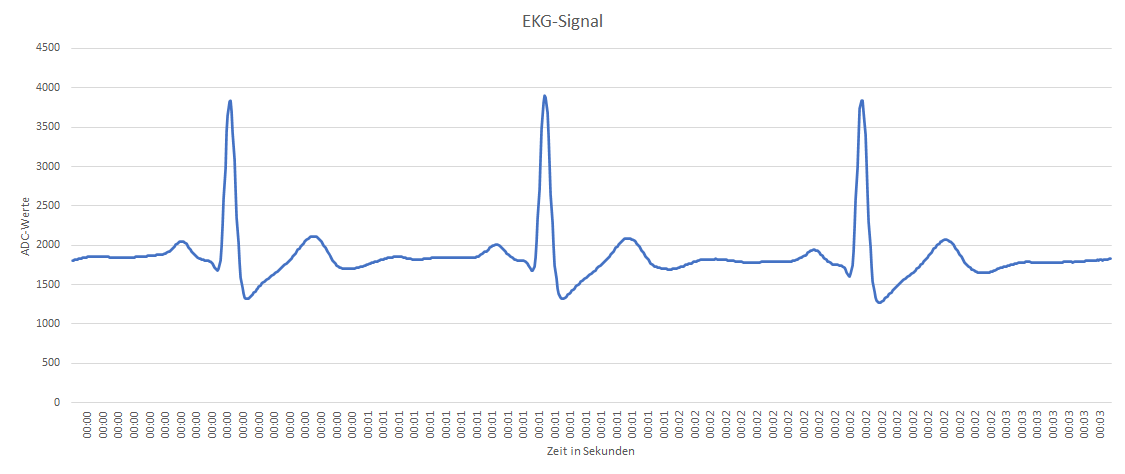
\includegraphics[width=\textwidth] {EKG_Endergebnis.png}
	\caption{aufgenommenes EKG-Signal}
	\label{Endergebnis EKG-Signal} 
\end{figure}

Gut zu erkennen sind die P- (Vorhofkontraktion) und die T-Welle (Erregungsrückbildung der Kammern). Zwischen den beiden Wellen befindet sich der QRS-Komplex. Deutlich von einander zu unterscheiden sind die negativen (Q- und S-Zacke) und positiven Anteile (R-Zacke) des Komplexes, der die Kammerkontraktion markiert. Im Signal sind keine störenden 50-Hz Schwingungen mehr enthalten. Aus den ADC-Werten lässt sich nun die Amplitude des Eingangssignals bei der Messung an der Hautoberfläche berechnen. Die Verstärkung der Filterschaltung wurde hierbei zur Vereinfachung als maximal (\SI{67}{\decibel}) über die gesamte Bandbreite angenommen. 

$$  \frac{\frac{ADC-Breite}{\textit{delta Signalwerte}} \cdot \textit{3 V}}{\textit{Verstärkung der Filterschaltung}} $$ 

Es ergibt sich eine Eingangsamplitude von \SI{2,1}{\milli\volt}, was der EKG-Amplitude eines gesunden Menschen in der Ableitung Einthoven 2 entspricht. Der Test der Langzeit-Aufnahme lieferte 21600000 Werte. Dies entspricht einer durchschnittlichen Abtastrate von \SI{250}{\hertz}. 

Die Funktion zur Berechnung der Herzfrequenz im Kurzzeit-EKG liefert eine gleichmäßiges Ausgangssignal. Zur Überprüfung wurde der Mittelwert der Herzfrequenz über eine Minute berechnet und mit dem analog gemessenen Puls am Handgelenk verglichen, wobei beide Werte übereinstimmten. Dies gilt jedoch nur für ein Ruhe-EKG, bei dem der Anwender sich möglichst wenig bewegt und gleichmäßig atmet. Bei Störungen von mehr als \SI{6}{\sec} Dauer, führen die Bewegungsartefakte zu einer Verfälschung der Pulsrate. 

\subsection{Akkulaufzeit, Bedienung, sonstige Funktionalität}

Für die verschiedenen Energiemodi wurde der Stromverbrauch direkt an der Batterie gemessen. Hierfür wurde ein Multimeter als Shunt zwischen den positiven Pol der Batterie und den positiven Eingangspin der Platine geschaltet.

\begin{table}
\center
\begin{tabular}[]{l|r}
\textbf{Modus} & \textbf{gemessener Strom} 
\\
\hline
\textbf{Display an / volle Helligkeit} & \SI{220}{\milli\ampere} 
\\
\hline
\textbf{Display im Sleep-Modus} & \SI{107}{\milli\ampere} 
\\
\hline
\textbf{5 V-DCDC ausgeschaltet} & \SI{7,7}{\milli\ampere}
\end{tabular}

\caption{Stromverbrauch}
\label{tab:Stromverbrauch}

\end{table}

Nach dem Test der Langzeitaufnahme (Gerät befand sich dafür fast ausschließlich im Energiesparmodus), mit einem anfangs vollen Akku, betrug die Akkuanzeige des Displays 61\%. Die Spannung der Akkuzelle gemessen mit dem Multimeter betrug \SI{3,83}{\volt}.

Die maximale Akkulaufzeit im Lagerzustand (5V DCDC ausgeschaltet) bis zur Entladegrenze von 20\% berechnet sich zu
$ \frac{2200\,mAh \cdot 0,8}{7,7\,mA} = 228,6\,h $.
%Akkustand beginnt bei 100\% und sinkt danach erwartungsgemäß bis bei einer Restladung von <20\% das akustische Warnsignal ertönt